\documentclass[11pt]{beamer}
\usetheme{Singapore}

\usepackage[utf8]{inputenc}
\usepackage[T1]{fontenc}
\usepackage{soul}
\usepackage{graphicx}


\graphicspath{{../Figures/}}

\def\et{{\it et al.}}


\author{Cody Glickman, Elaine Epperson, and Michael Strong \\ BRASS 2018}

\title{Environmental Microbiome of Asthmatic Homes}

%\subtitle{}
%\logo{}

\date{ 
\includegraphics[height=2cm, width=2cm]{lablogo.png} \\ June, 2018}
%\subject{}
\setbeamercovered{transparent}
\setbeamertemplate{navigation symbols}{}
\setbeamertemplate{theorems}[numbered]

\begin{document}
	\maketitle

	%--------------------------------------------------------------------------------------

	
\section{Introduction}
\subsection{}

	\begin{frame}{Microbiome}
		\begin{block}{Definition}
		The community composition of microorganisms in a niche
		\end{block}
		
		\begin{columns}
		\column{0.5\textwidth}
		\begin{block}{Capabilities of Microbiome}
		\begin{itemize}
		\item Diversity of niche
		\item Relationships between samples
		\item Composition of niche
		\end{itemize}
		\end{block}
		
		\column{0.5\textwidth}
		\begin{block}{Limitations of Microbiome}
		\begin{itemize}
		\item Relative abundances
		\item Functional information is missing
		\item Sequencing length limits depth of taxonomic classification

		\end{itemize}
		\end{block}
		
		\end{columns}
	
	\end{frame}
	%--------------------------------------------------------------------------------------
	
	\begin{frame}{Microbiome Sequencing Methods}
	\begin{columns}
	\column{0.5\textwidth}
	\begin{block}{Conserved Universal Gene}
	16S ribosomal RNA: \\
	A genetic element found across all prokaryotes 
	\end{block}
	
	\begin{block}{Regions of 16S}
	Contains alternating segments of conserved and hypervariable regions allowing for amplification and differentiation
	\end{block}
	
	\column{0.5\textwidth}
	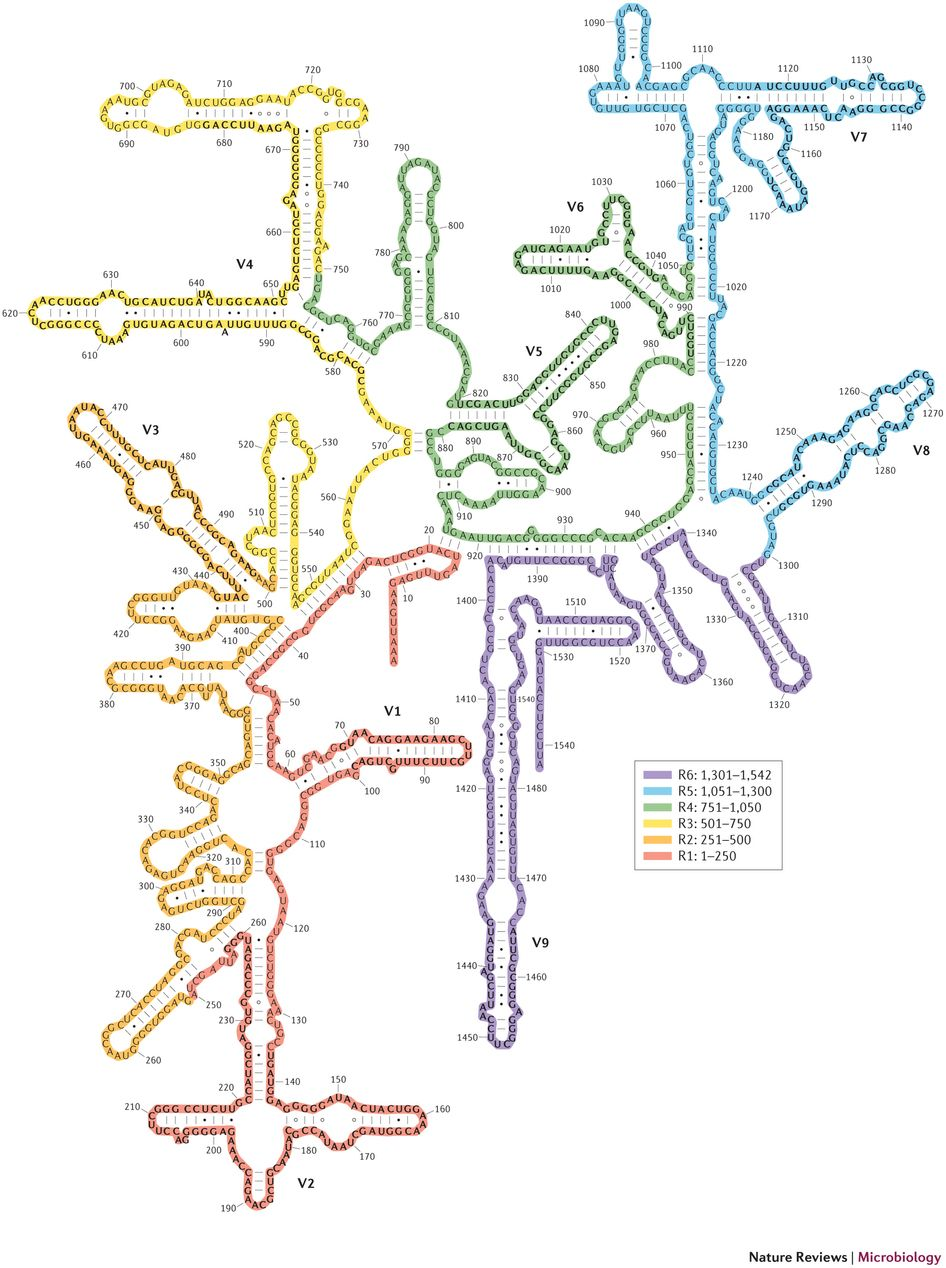
\includegraphics[height=6cm, width=5cm]{16S.jpg} \\
	\hspace{0.5cm}	
	\tiny{Yarza, P, et al. (2014)}
	\end{columns}

	
	\end{frame}

	
\section{Methods}
\subsection{}


	%-----------------------------------------	
	\begin{frame}{BRASS Data Collection}
	\begin{columns}
	\column{0.5\textwidth}
	\begin{block}{BRASS Study Swabs (76 total)}
		\begin{itemize}
			\item Swabs from 7 patients' homes
			\item 1 to 3 visits per patient
			\item 7 study sites
		\end{itemize}
	\end{block}
	\begin{block}{16S Sequencing}
	\begin{itemize}
		\item Reads generated on Illumina MiSeq
		\item More than 12 Million Paired End Reads
	\end{itemize}
	\end{block}
	
	
	\column{0.5\textwidth}
	\begin{block}{Read Distribution}
	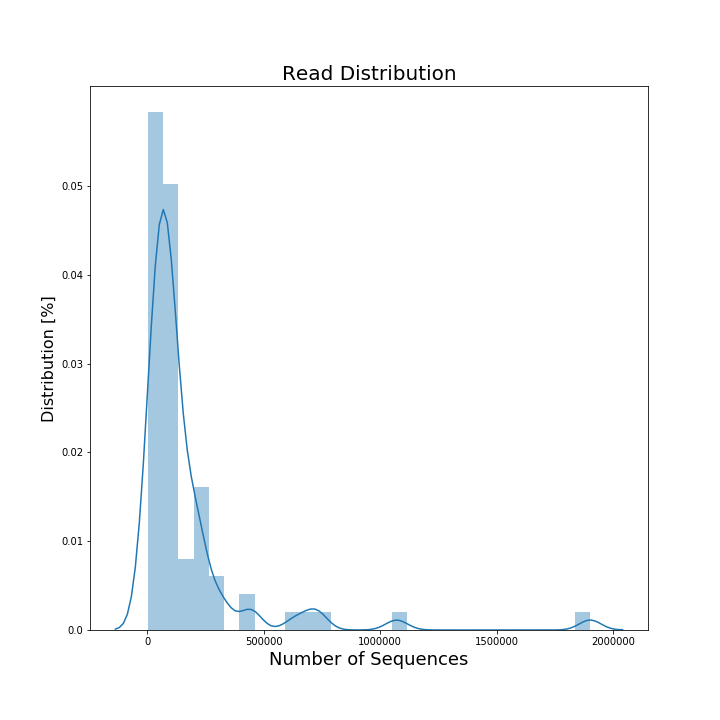
\includegraphics[height=3cm, width=4cm]{brass_histo.png}\\
	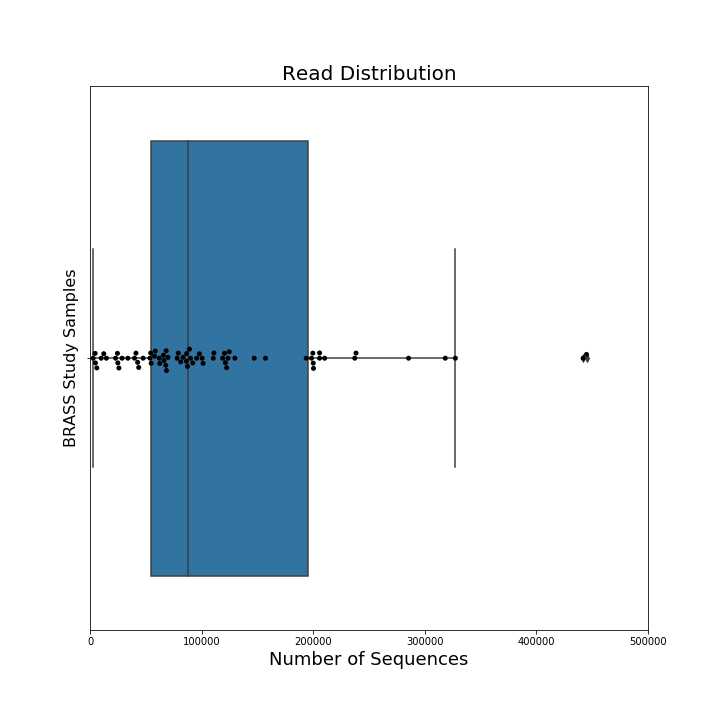
\includegraphics[height=3cm, width=4cm]{brass_boxplot.png}
	\end{block}
	\end{columns}
	\end{frame}

	%-----------------------------------------	
	
	\begin{frame}{Qiime2 Workflow}
	\begin{columns}
	\column{0.4\textwidth}
	\hspace{2cm}
	\begin{block}{Operations}
	\begin{itemize}
	\item \alert{Illumina error correction}
	
	
	\definecolor{blues}{rgb}{0.2, 0.2, 0.6}
	\color{blues}
	\item Taxnomic assignment
	
	\definecolor{amber}{rgb}{1.0, 0.49, 0.0}
	\color{amber}
	\item Diversity metrics
  \end{itemize}
  \end{block}
  
	\column{0.7\textwidth}
	\centering
	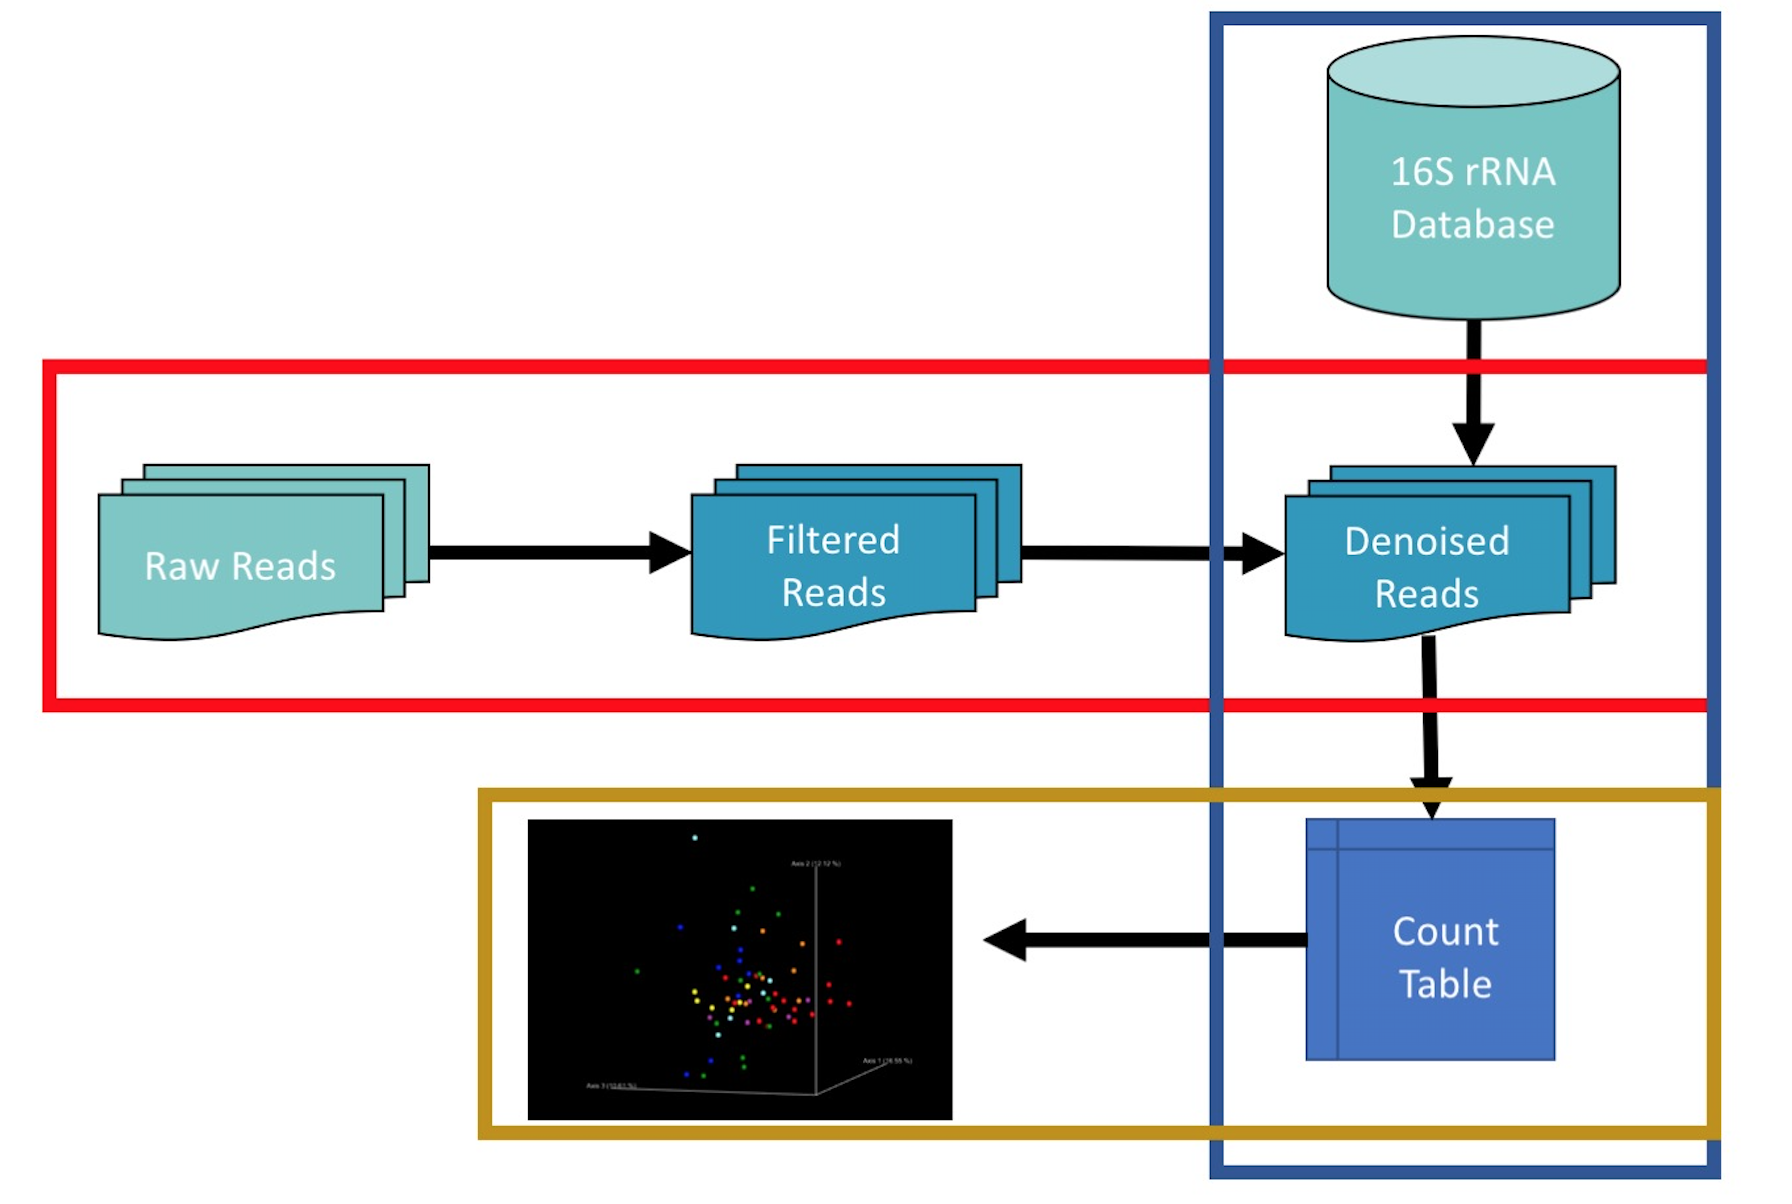
\includegraphics[height=7cm, width=6cm]{qiime_workflow.png}
	\end{columns}
	\end{frame}
	
	%-----------------------------------------
	
	\begin{frame}{Illumina Error Correction}
	\centering
	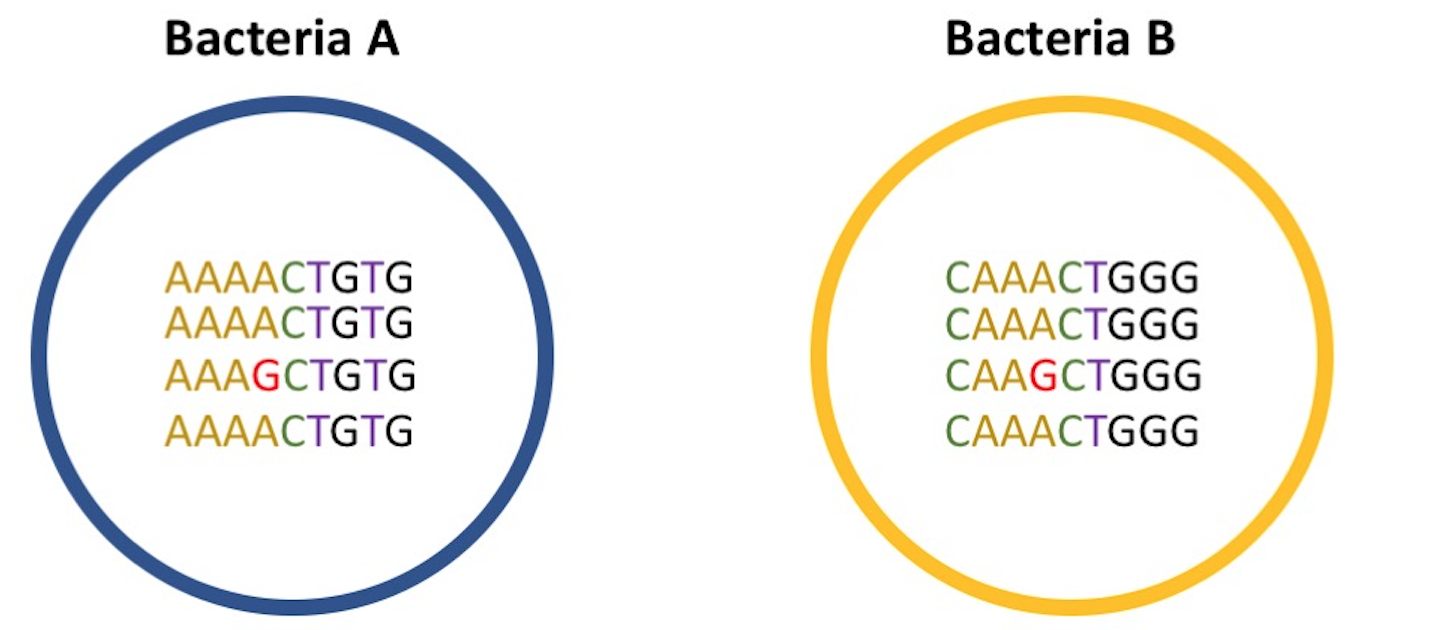
\includegraphics[height=4cm, width=8cm]{Error1.png}
	\end{frame}
	
	\begin{frame}{Illumina Error Correction}
	\centering
	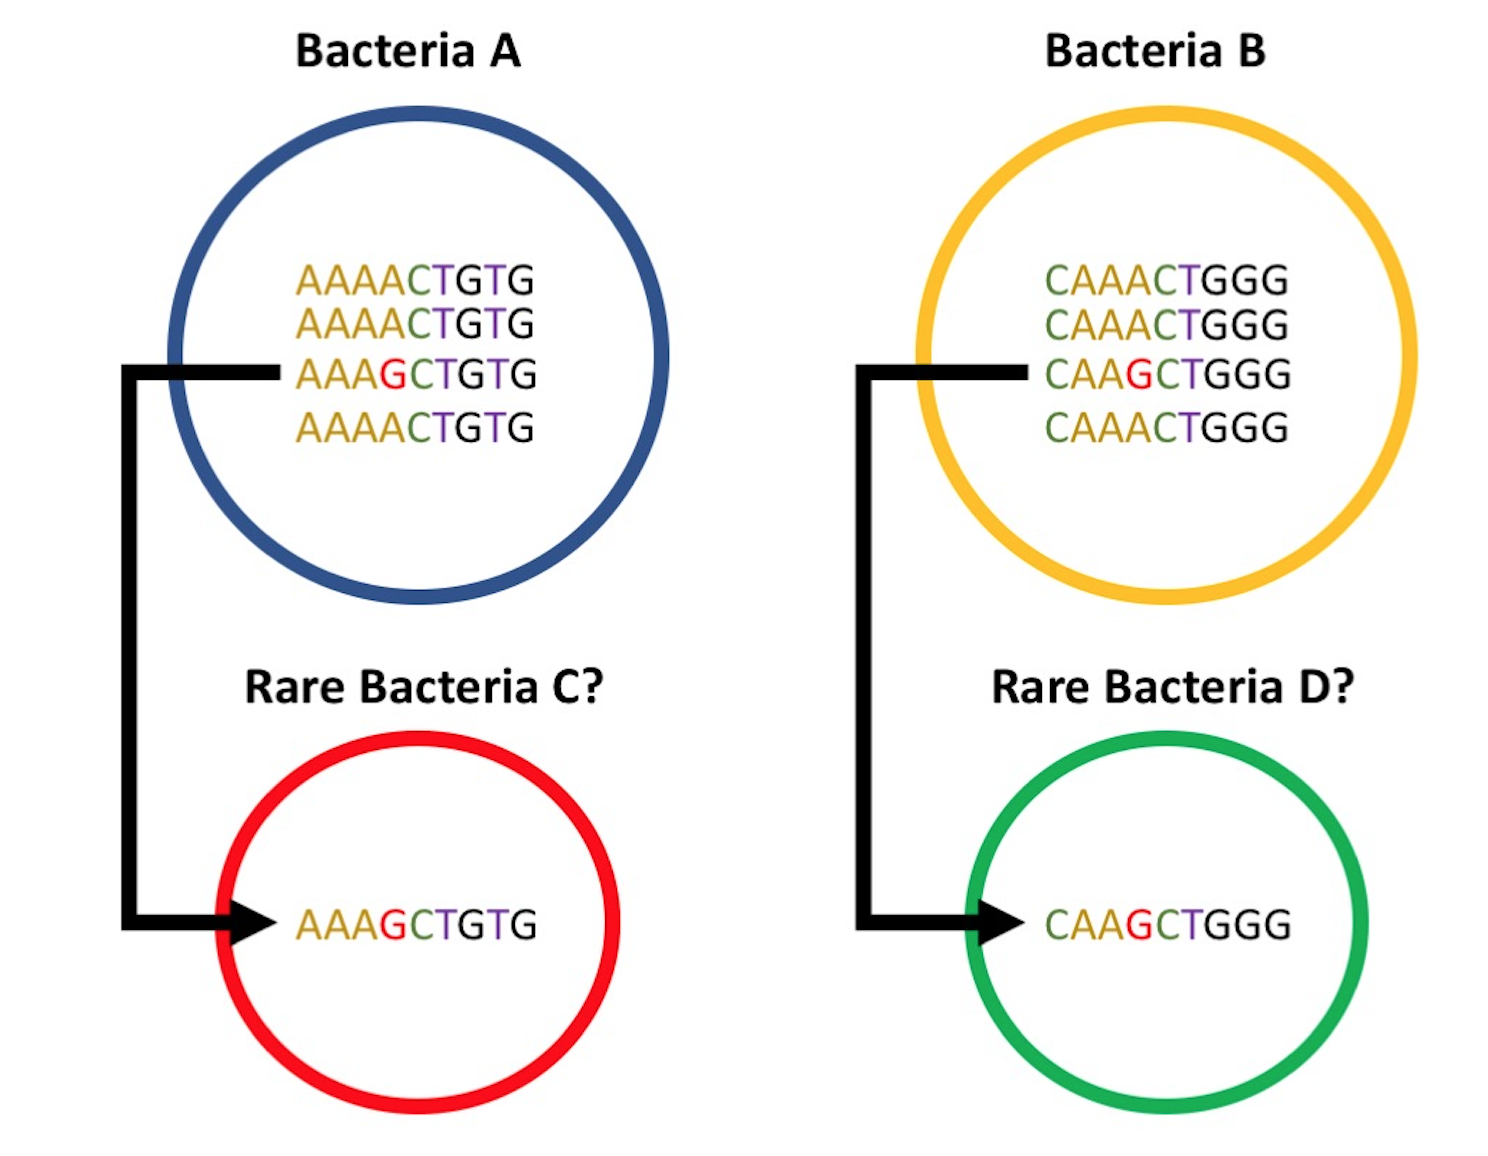
\includegraphics[height=7cm, width=7cm]{Error2.png}
	\end{frame}
	
	%-----------------------------------------
	
	
	\begin{frame}{Workflows}
	\begin{block}{Illumina Error Correction}
	\end{block}
	\centering
	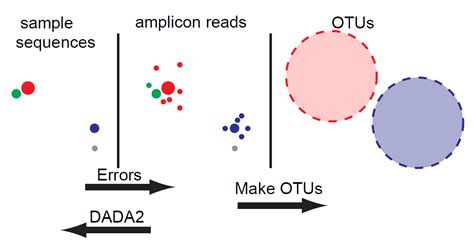
\includegraphics[height=7cm, width=10cm]{DADA.jpg}
	\hspace{-2cm}
	
	\end{frame}
	
		%-----------------------------------------
		
	\begin{frame}{Workflows}

	\begin{block}{Taxonomic Assignment}
	\end{block}
	\begin{columns}
	\column{0.6\textwidth}
	\begin{block}{Taxonomy Classifier}
	Assign raw reads with a Naive Bayes classifer trained on 16S Database
	\end{block}
	
	\begin{block}{16s rRNA Databases}
	
	GreenGenes 
	\\
	Silva 132 (Troubleshooting)
	
	\end{block}

	
	
	\column{0.4\textwidth}
	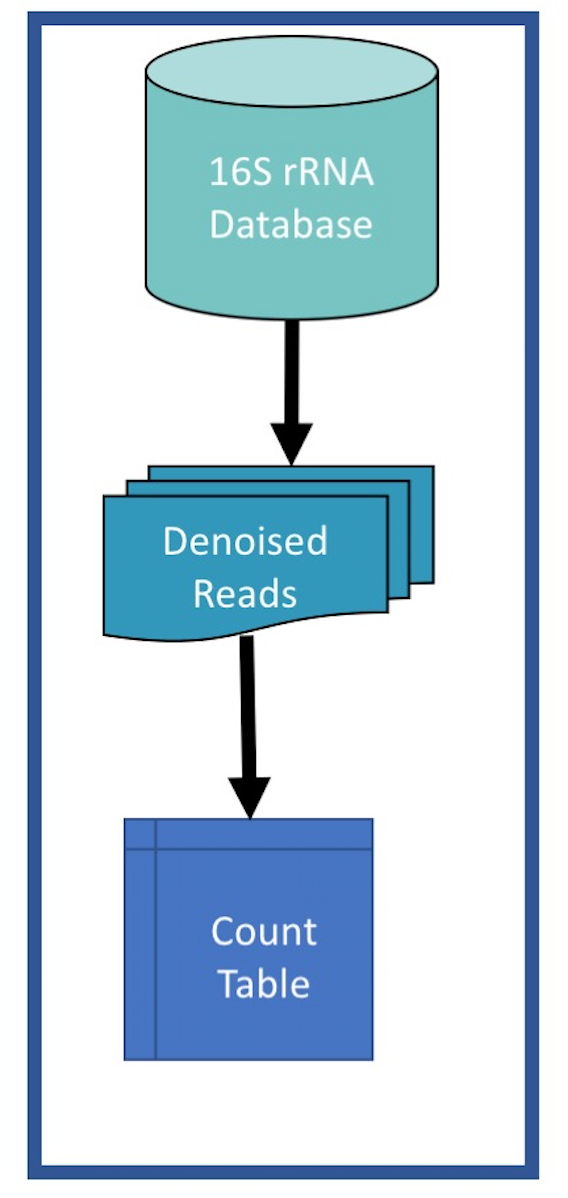
\includegraphics[height=5cm, width=4cm]{classifer.png}
	
	
	
	\end{columns}
	\end{frame}
	
	
	
\section{Results}
\subsection{}
	%-----------------------------------------	
	
	
	
	\begin{frame}{Diversity Metrics}
	\begin{columns}
	\column{0.4\textwidth}
	\hspace{2cm}
	\begin{block}{Alpha Diversity}
	Richness or organismal diversity of samples
	\begin{itemize}
	\item Faith's Phylogenic Diversity \\ 
	Tree Based Alpha Diversity Estimate
	
	\item Shannon Diversity Index\\
	$H = -\sum[(p_i) * ln(p_i)]$
  $E=H/H_max$
  $SI = \sum[E_i]$
  
  
  \end{itemize}
  \end{block}
  
	\column{0.7\textwidth}
	\centering
	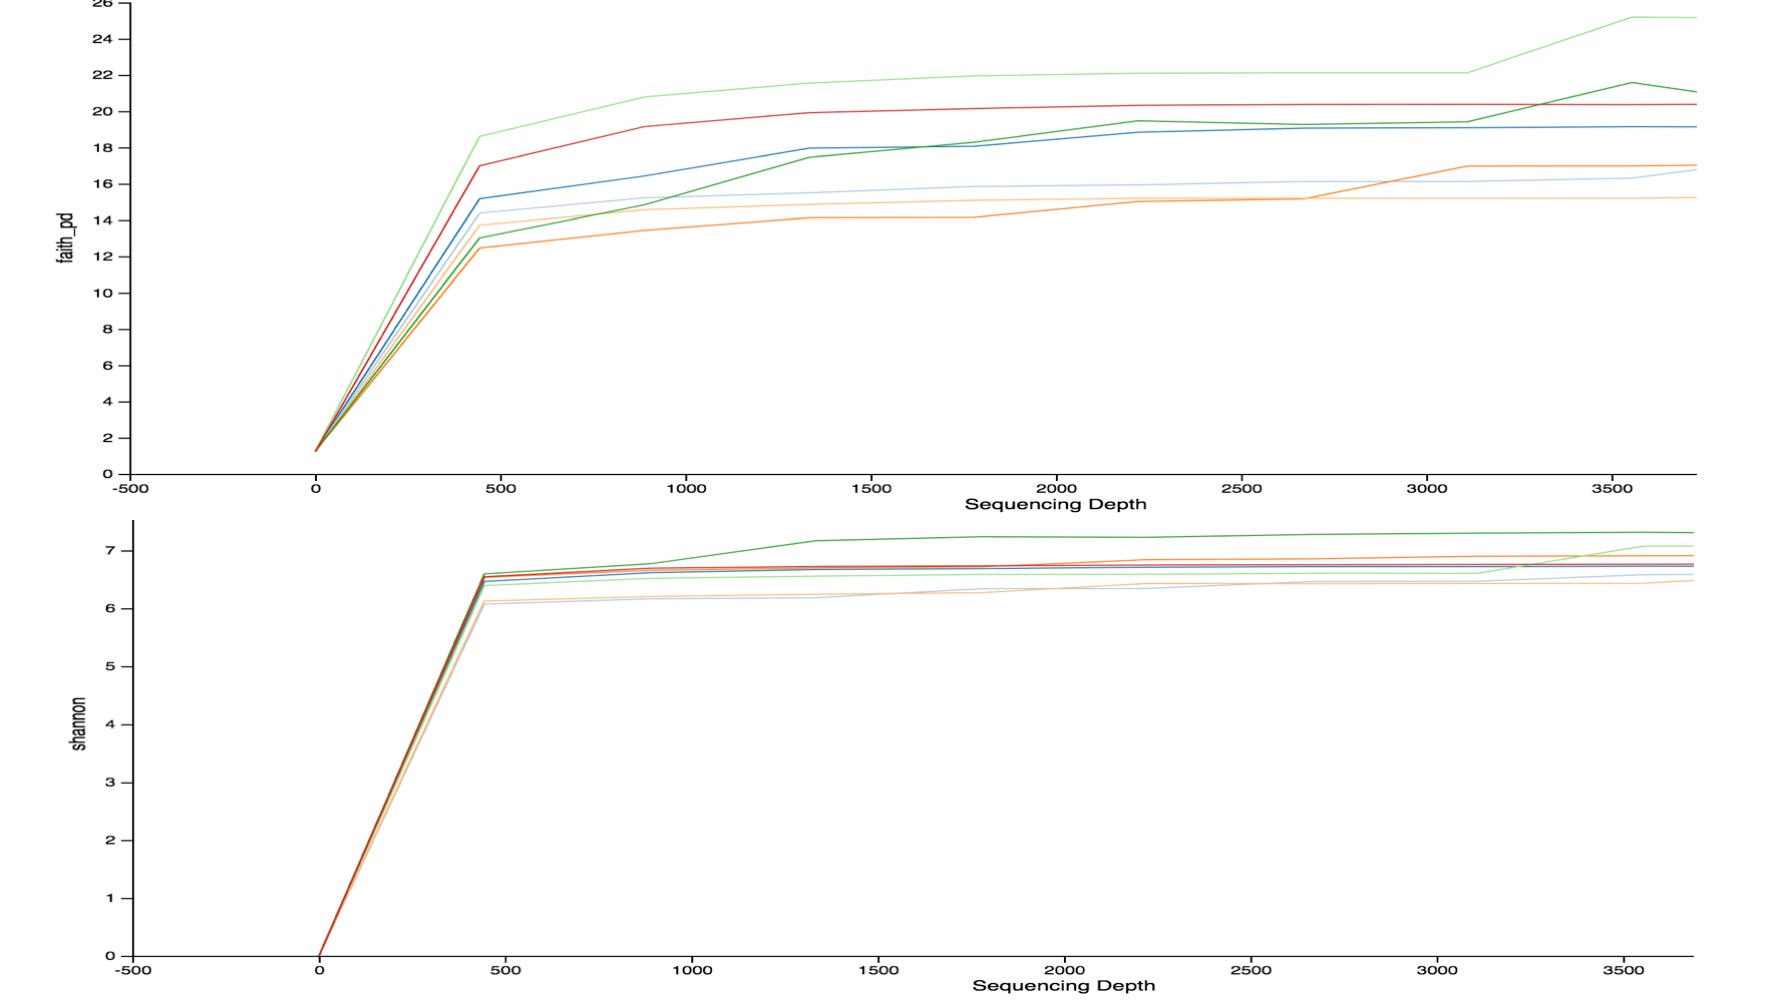
\includegraphics[height=8cm, width=6cm]{alpha.jpg}
	\end{columns}
	\end{frame}
	
	\begin{frame}{Diversity Metrics (Alpha Diversity Barplots)}
	\centering
	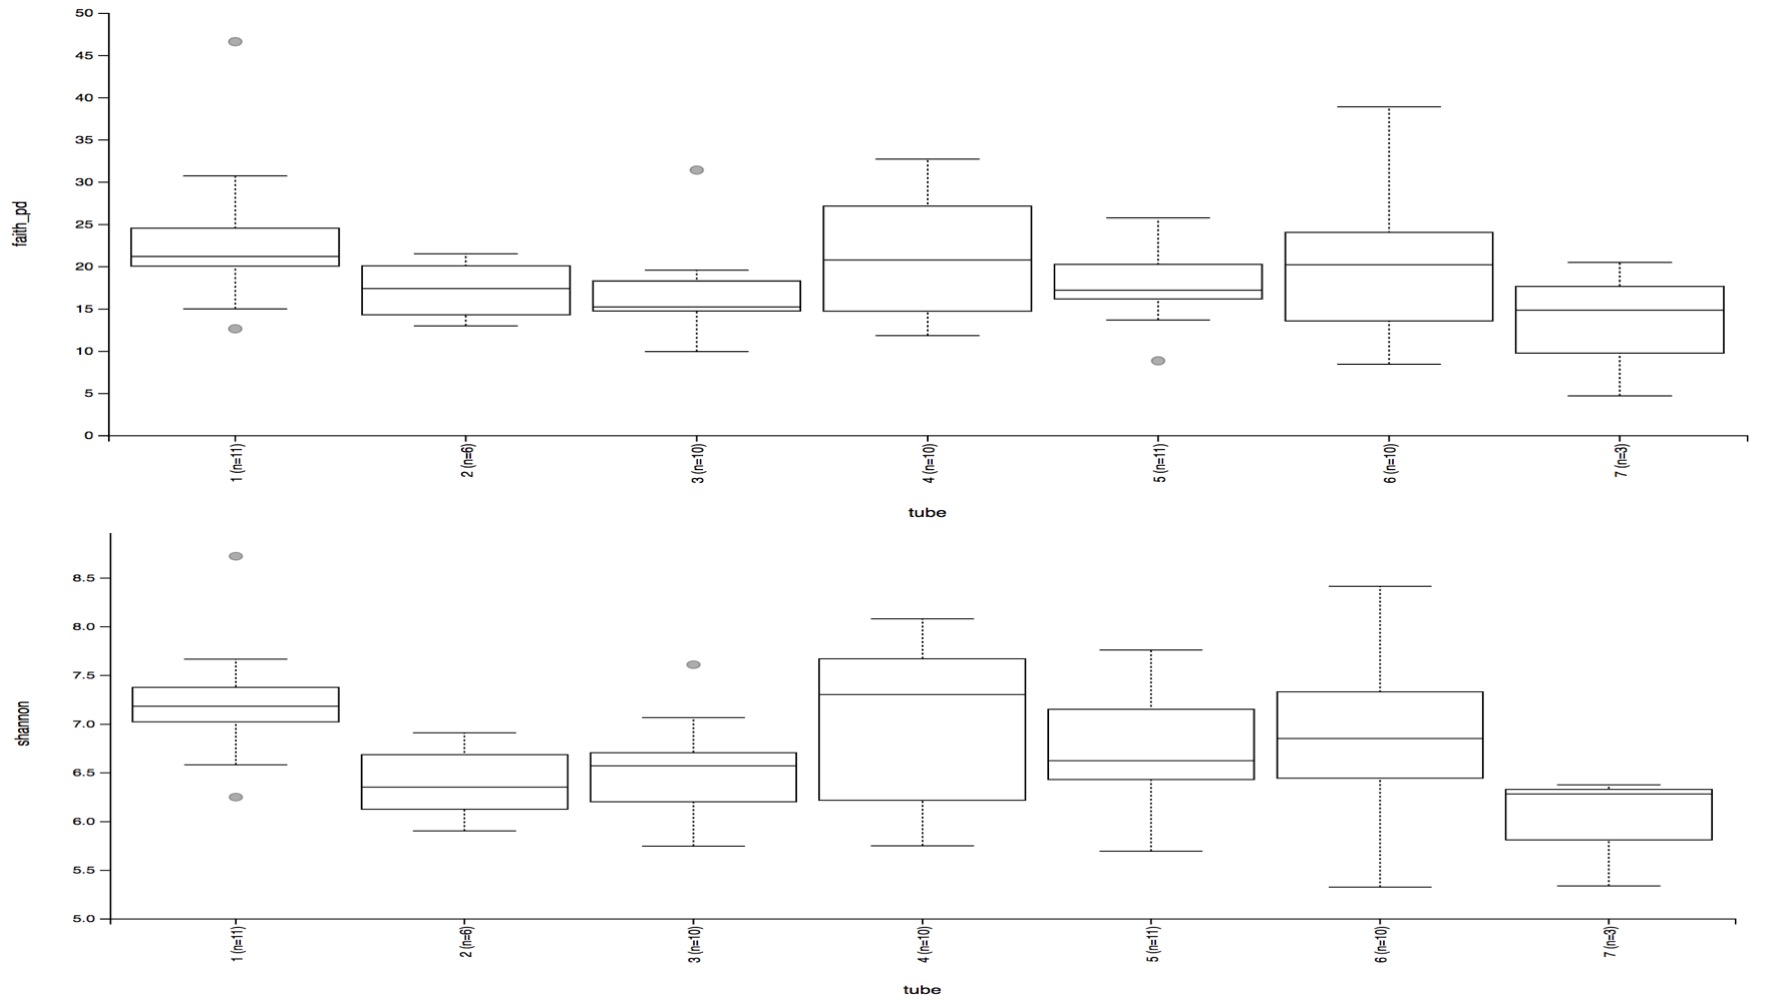
\includegraphics[height=8cm, width=12cm]{Tube.jpg}
	\end{frame}
	%-----------------------------------------	
	\begin{frame}{Diversity Metrics}
	\begin{block}{Beta Diversity}
	Evenness or distances of counts between samples
	\end{block}
	\begin{columns}
	\column{0.4\textwidth}
	\hspace{2cm}
	\begin{block}{Weight Unifrac}
  Measure takes into account abundances and phylogeny 
  \end{block}
  
  \begin{block}{PERMANOVA}
  Distances within a group is more similar to each other than outside group
  \end{block}
  
  \begin{block}{Significance}
	By House: p < 0.001
	\\
	By Tube: p < 0.001
	\end{block}
	
	\column{0.6\textwidth}
	\centering
	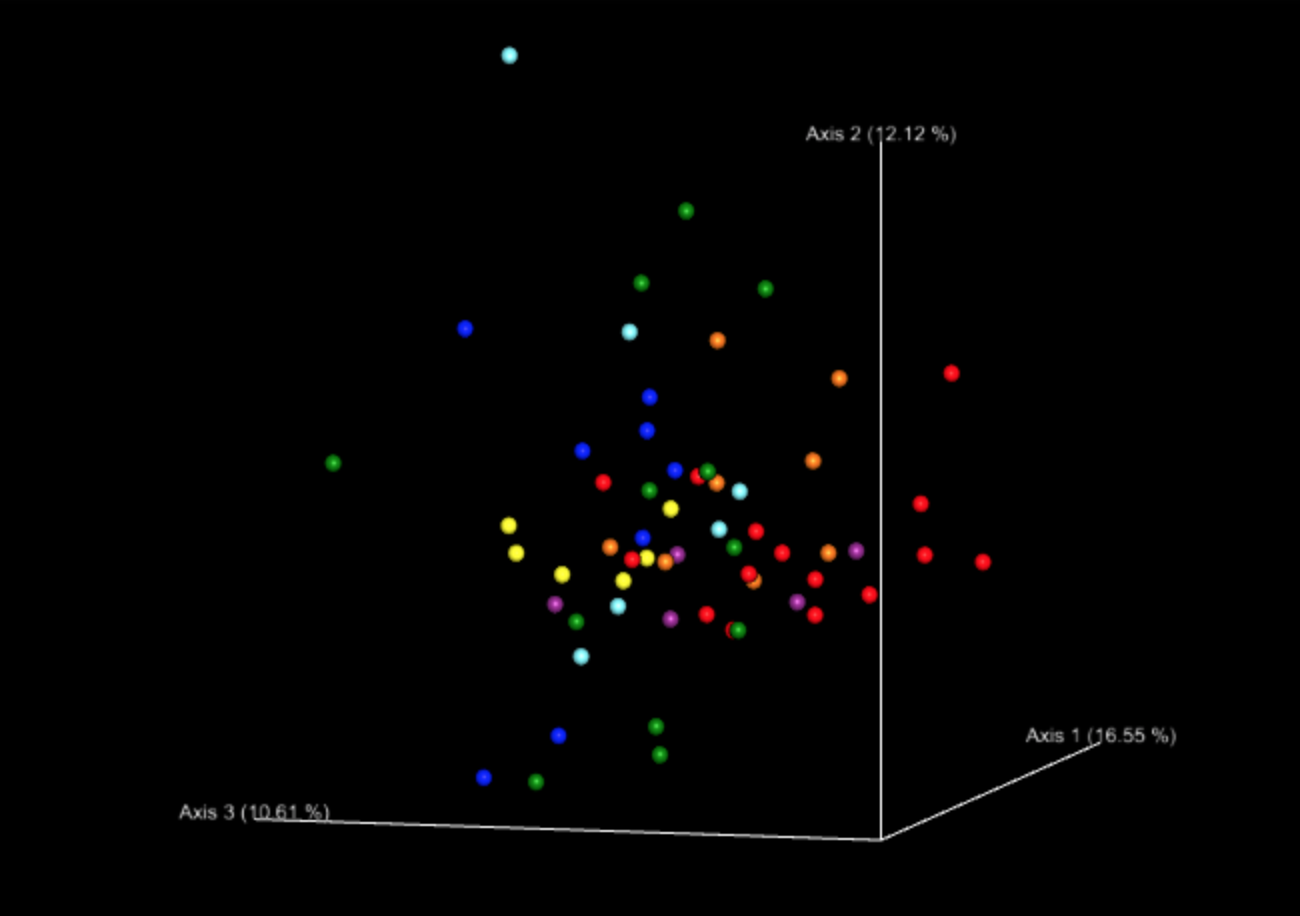
\includegraphics[height=6cm, width=8cm]{Beta_Diversity.png}
	\end{columns}
	
	

	\end{frame}
	
		%-----------------------------------------	
	\begin{frame}{Diversity Metrics (Taxa Bar Plots)}
	\centering
	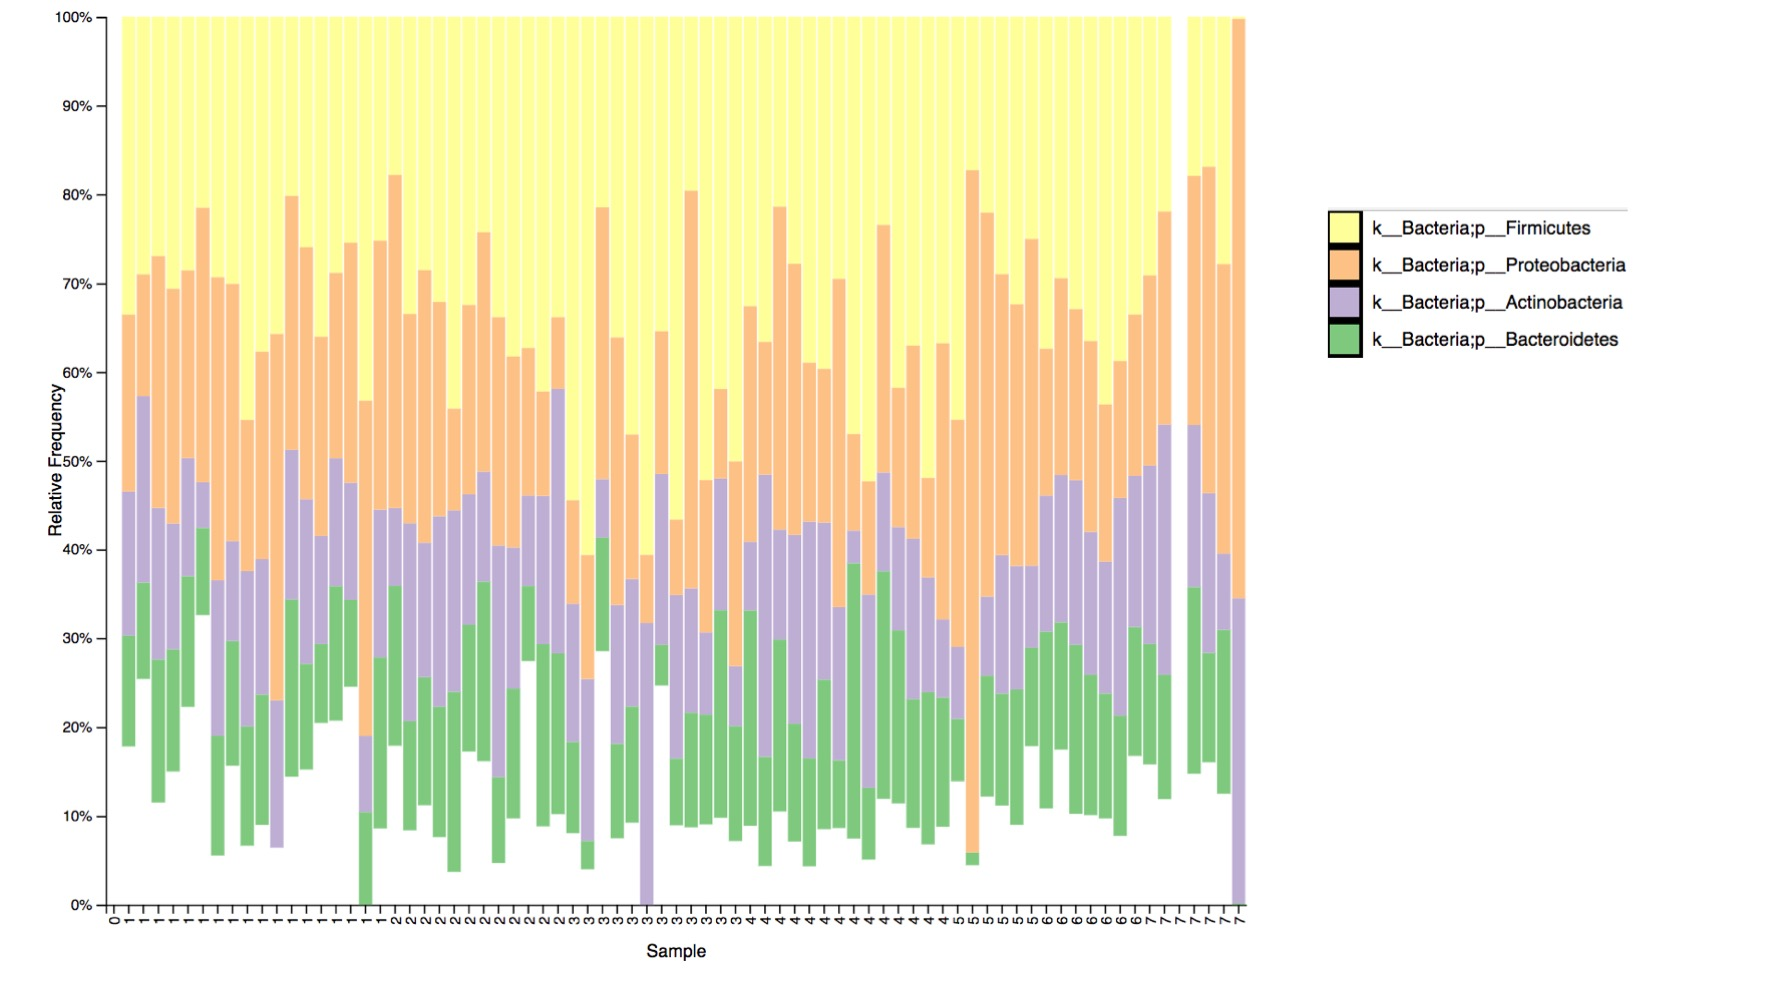
\includegraphics[height=8cm, width=12.5cm]{phylum.jpg}
	
	\end{frame}
	
	

\section{}

	
	%-----------------------------------------	
	\begin{frame}{Acknowledgements}
	\centering
	{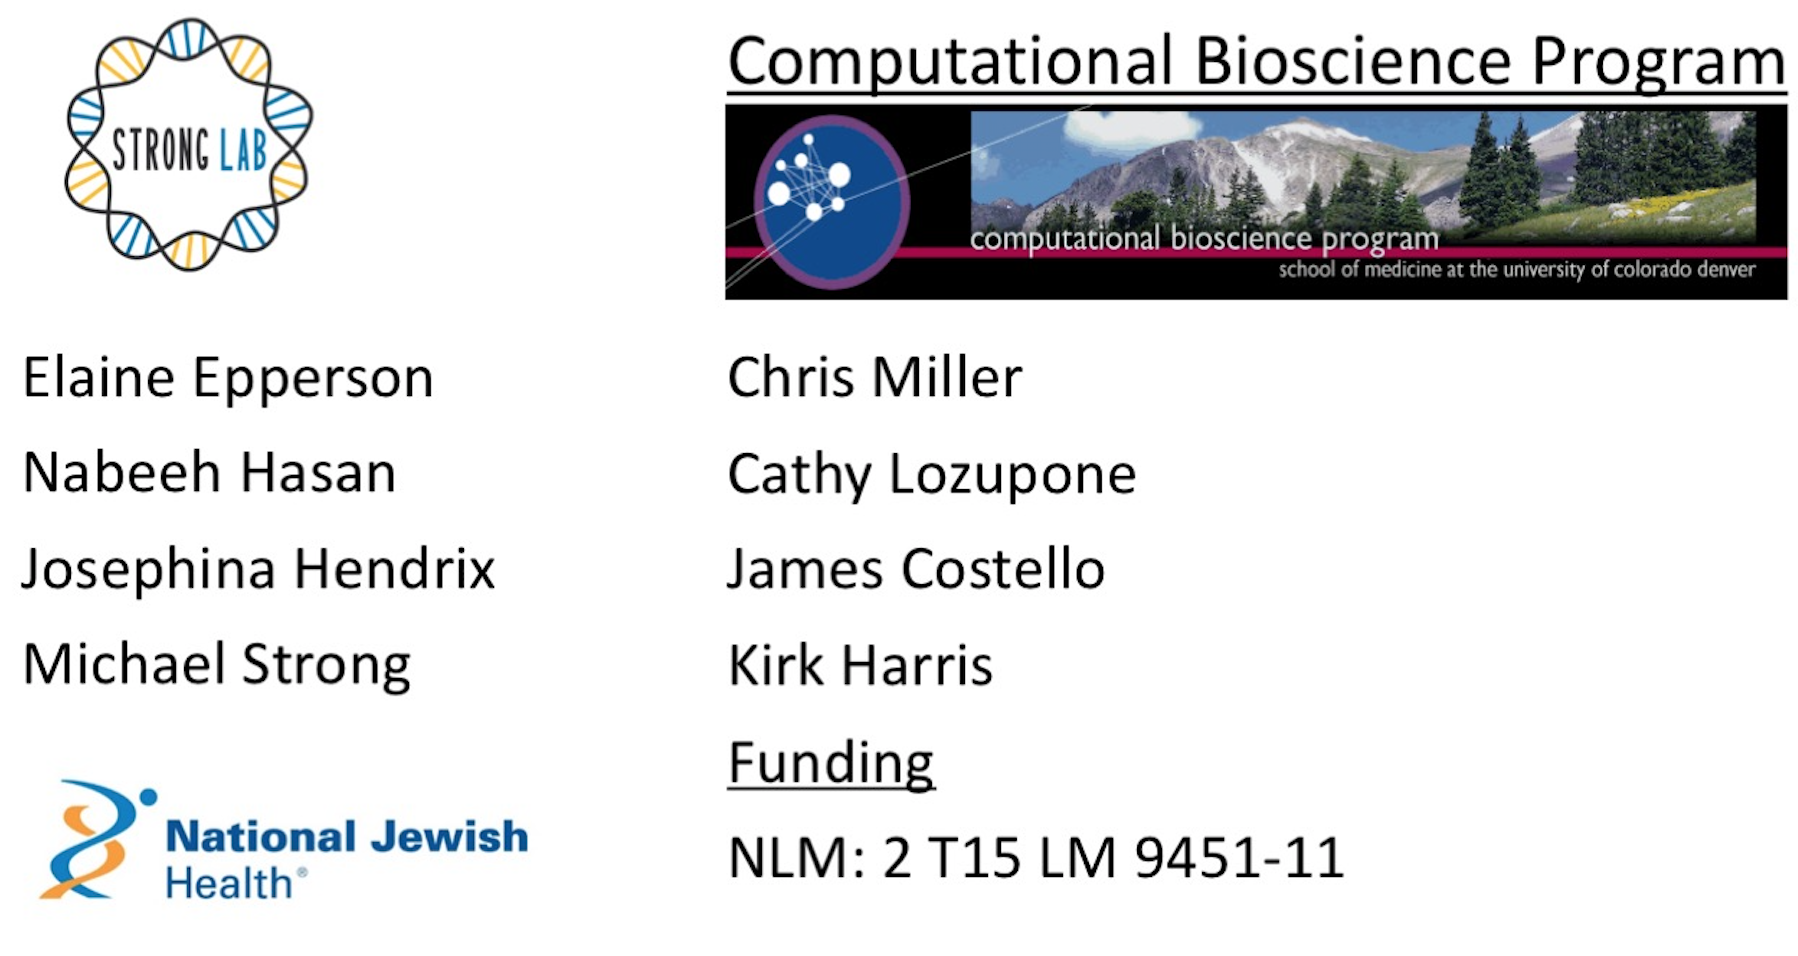
\includegraphics[height=5cm, width=11cm]{Acknowledgements.png} }
	\end{frame}
	
	%-----------------------------------------	
	\begin{frame}{Questions?}
	\center
	Cody Glickman \\ 
\includegraphics[height=2cm, width=2cm]{lablogo.png} \\ cody.glickman@ucdenver.edu \\ \alert{www.github.com/glickmac} \\ www.codyglickman.com
	\end{frame}


\end{document}